\documentclass[11pt]{article}
\usepackage[textwidth=18.0cm, textheight=23.0cm, top=2.0cm]{geometry}
\usepackage{pst-all}
\usepackage{amssymb}
\usepackage{tikz}
\usepackage{underscore}\begin{document}
\pagestyle{empty}


ClassName: \underline{\textbf{Class_08.2bp-2}}
\par
BinSize: \underline{\textbf{100 × 100}}
\par
ReduceSize: \underline{\textbf{100 × 100}}
\par
TypeNum: \underline{\textbf{20}}
\par
Num: \underline{\textbf{20}}
\par
OutS: \underline{\textbf{50000}}
\par
InS: \underline{\textbf{44102}}
\par
Rate: \underline{\textbf{0.882}}
\par
UB: \underline{\textbf{5}}
\par
LB0: \underline{\textbf{5}}
\par
LB: \underline{\textbf{5}}
\par
LBWithCut: \underline{\textbf{5}}
\par
NodeCut: \underline{\textbf{0}}
\par
ExtendedNodeCnt: \underline{\textbf{1}}
\par
GenNodeCnt: \underline{\textbf{1}}
\par
PrimalNode: \underline{\textbf{0}}
\par
ColumnCount: \underline{\textbf{5}}
\par
TotalCutCount: \underline{\textbf{0}}
\par
RootCutCount: \underline{\textbf{0}}
\par
LPSolverCnt: \underline{\textbf{1}}
\par
PricingSolverCnt: \underline{\textbf{0}}
\par
BranchAndBoundNum: \underline{\textbf{1}}
\par
isOpt: \underline{\textbf{true}}
\par
TimeOnInitSolution: \underline{\textbf{600.000 s}}
\par
TimeOnPrimal: \underline{\textbf{0.000 s}}
\par
TimeOnPricing: \underline{\textbf{0.000 s}}
\par
TimeOnRmp: \underline{\textbf{0.062 s}}
\par
TotalTime: \underline{\textbf{600.297 s}}
\par
\newpage


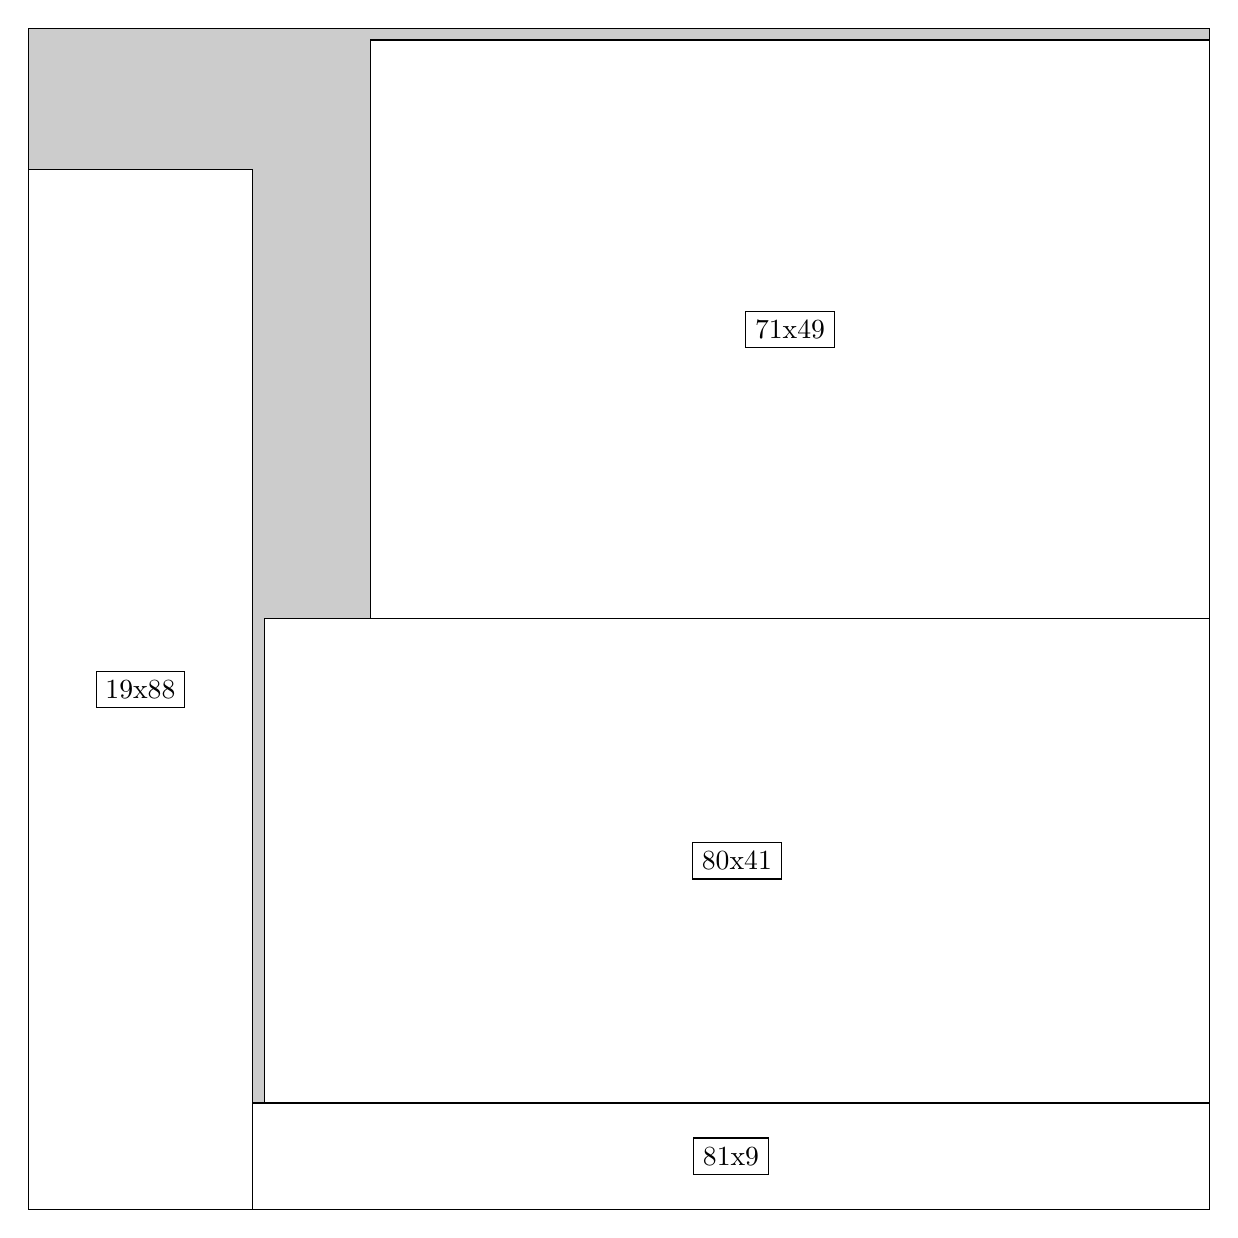
\begin{tikzpicture}[shorten >=1pt,scale=1.0,every node/.style={scale=1.0},->]
\tikzstyle{vertex}=[circle,fill=black!25,minimum size=14pt,inner sep=0pt]
\filldraw[fill=gray!40!white, draw=black] (0,0) rectangle (15.0,15.0);
\foreach \name/\x/\y/\w/\h in {81x9/2.85/0.0/12.15/1.3499999999999999,80x41/3.0/1.3499999999999999/12.0/6.1499999999999995,71x49/4.35/7.5/10.65/7.35,19x88/0.0/0.0/2.85/13.2}
\filldraw[fill=white!40!white, draw=black] (\x,\y) rectangle node[draw] (\name) {\name} ++(\w,\h);
\end{tikzpicture}


w =81 , h =9 , x =19 , y =0 , v =729
\par
w =80 , h =41 , x =20 , y =9 , v =3280
\par
w =71 , h =49 , x =29 , y =50 , v =3479
\par
w =19 , h =88 , x =0 , y =0 , v =1672
\par
\newpage


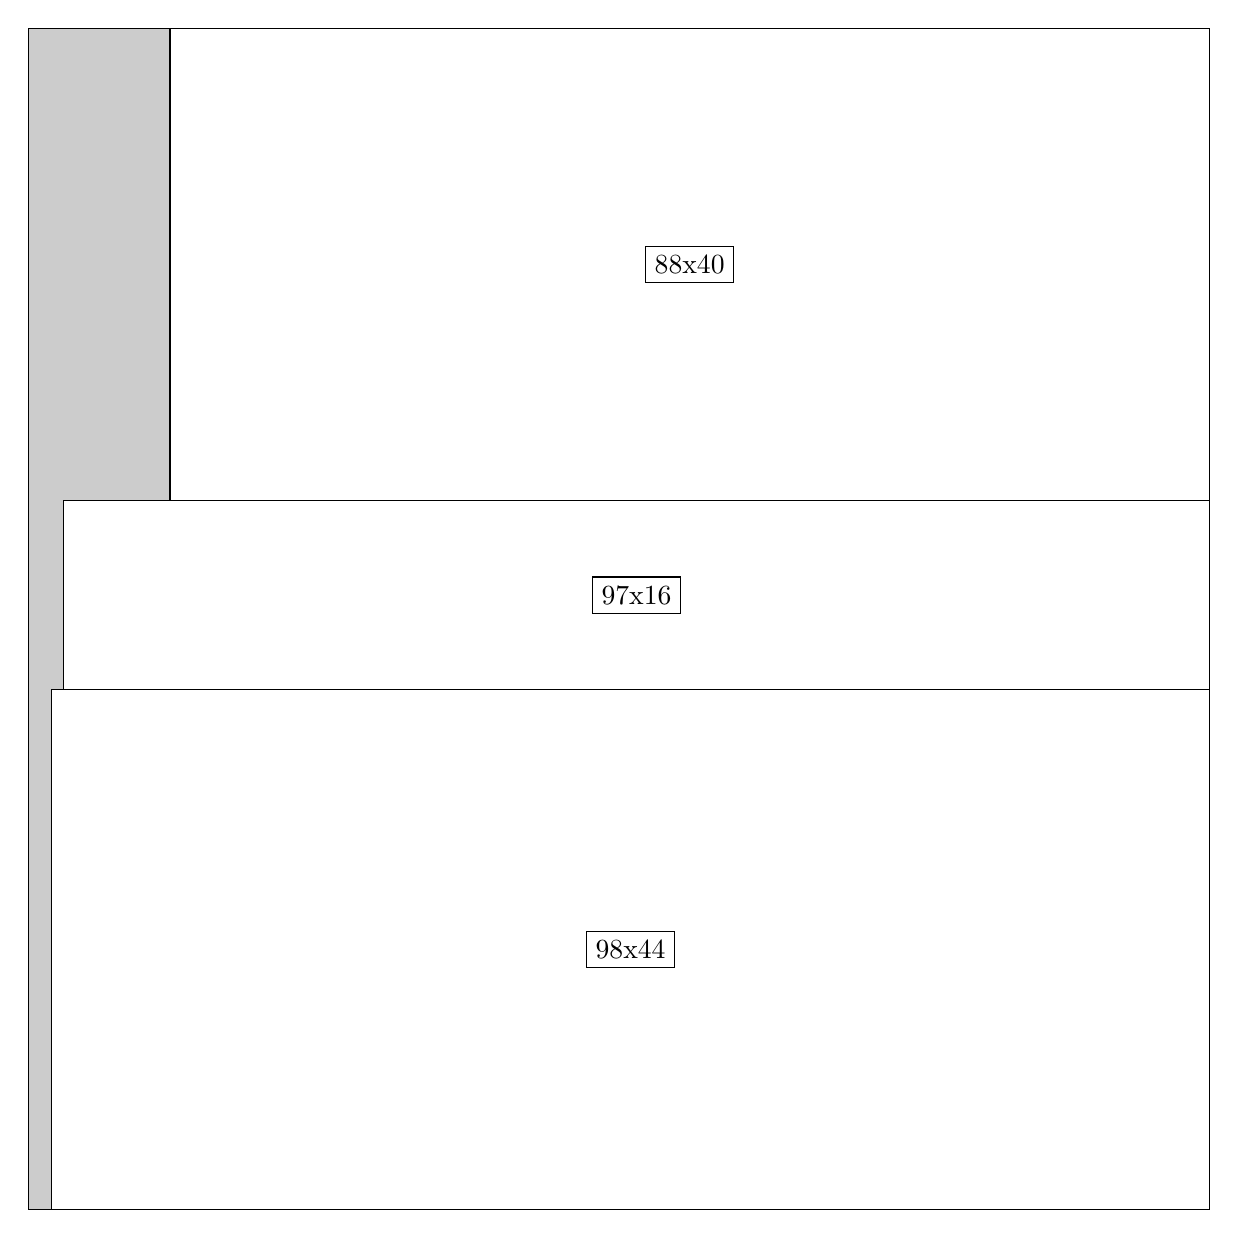
\begin{tikzpicture}[shorten >=1pt,scale=1.0,every node/.style={scale=1.0},->]
\tikzstyle{vertex}=[circle,fill=black!25,minimum size=14pt,inner sep=0pt]
\filldraw[fill=gray!40!white, draw=black] (0,0) rectangle (15.0,15.0);
\foreach \name/\x/\y/\w/\h in {98x44/0.3/0.0/14.7/6.6,97x16/0.44999999999999996/6.6/14.549999999999999/2.4,88x40/1.7999999999999998/9.0/13.2/6.0}
\filldraw[fill=white!40!white, draw=black] (\x,\y) rectangle node[draw] (\name) {\name} ++(\w,\h);
\end{tikzpicture}


w =98 , h =44 , x =2 , y =0 , v =4312
\par
w =97 , h =16 , x =3 , y =44 , v =1552
\par
w =88 , h =40 , x =12 , y =60 , v =3520
\par
\newpage


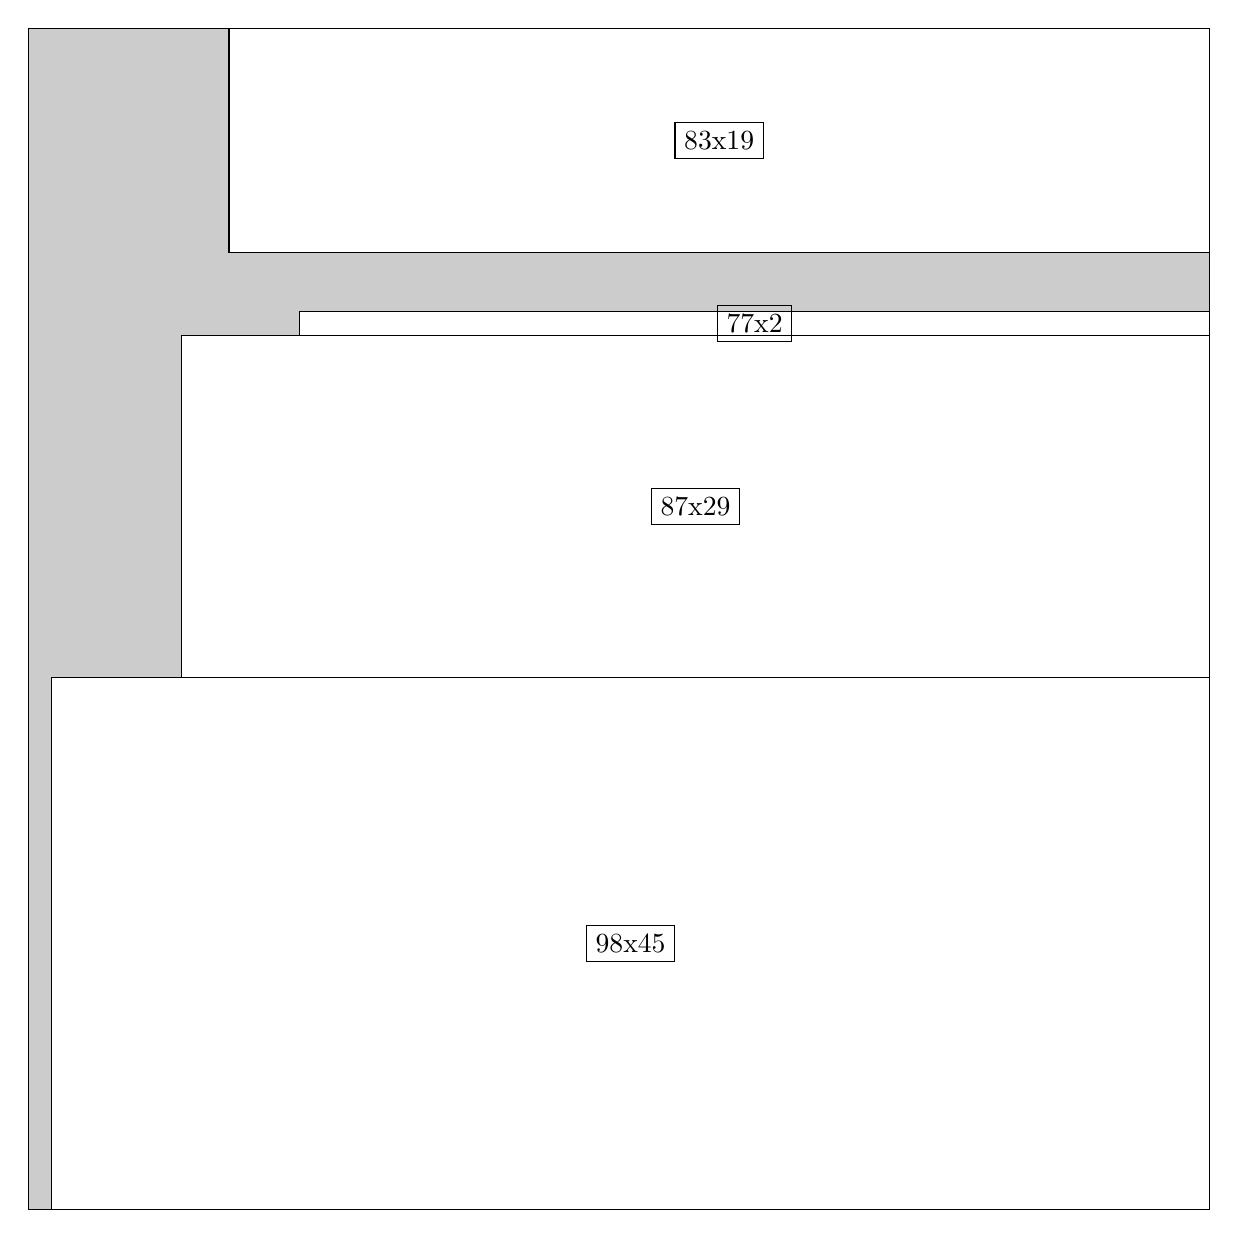
\begin{tikzpicture}[shorten >=1pt,scale=1.0,every node/.style={scale=1.0},->]
\tikzstyle{vertex}=[circle,fill=black!25,minimum size=14pt,inner sep=0pt]
\filldraw[fill=gray!40!white, draw=black] (0,0) rectangle (15.0,15.0);
\foreach \name/\x/\y/\w/\h in {98x45/0.3/0.0/14.7/6.75,87x29/1.95/6.75/13.049999999999999/4.35,77x2/3.4499999999999997/11.1/11.549999999999999/0.3,83x19/2.55/12.15/12.45/2.85}
\filldraw[fill=white!40!white, draw=black] (\x,\y) rectangle node[draw] (\name) {\name} ++(\w,\h);
\end{tikzpicture}


w =98 , h =45 , x =2 , y =0 , v =4410
\par
w =87 , h =29 , x =13 , y =45 , v =2523
\par
w =77 , h =2 , x =23 , y =74 , v =154
\par
w =83 , h =19 , x =17 , y =81 , v =1577
\par
\newpage


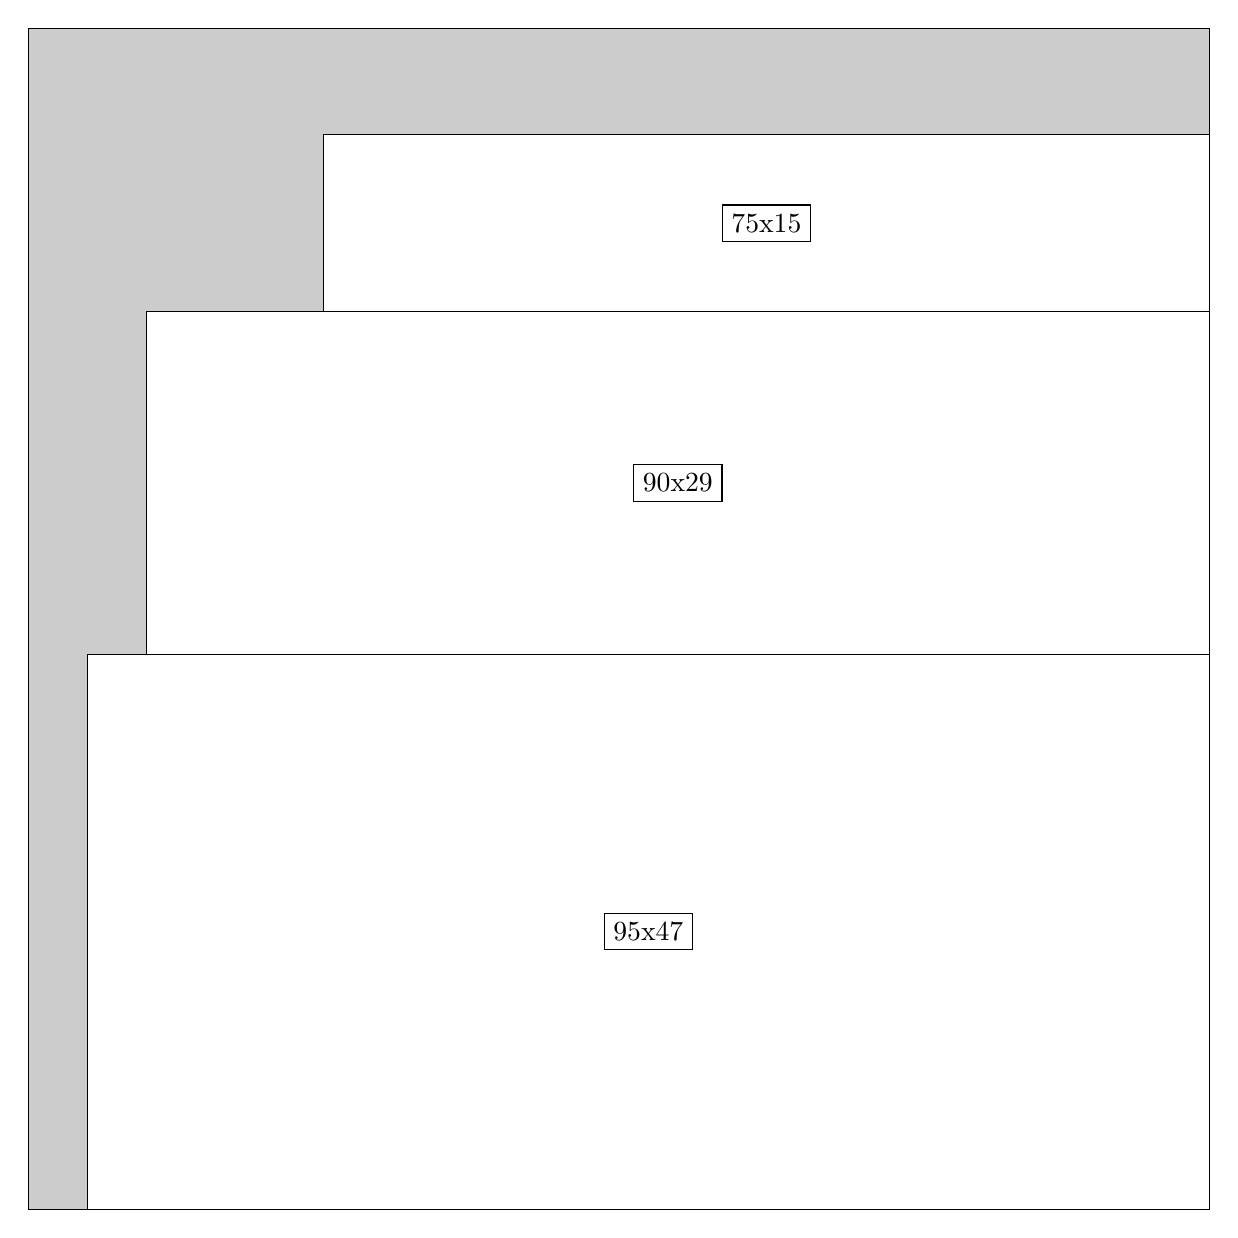
\begin{tikzpicture}[shorten >=1pt,scale=1.0,every node/.style={scale=1.0},->]
\tikzstyle{vertex}=[circle,fill=black!25,minimum size=14pt,inner sep=0pt]
\filldraw[fill=gray!40!white, draw=black] (0,0) rectangle (15.0,15.0);
\foreach \name/\x/\y/\w/\h in {95x47/0.75/0.0/14.25/7.05,90x29/1.5/7.05/13.5/4.35,75x15/3.75/11.4/11.25/2.25}
\filldraw[fill=white!40!white, draw=black] (\x,\y) rectangle node[draw] (\name) {\name} ++(\w,\h);
\end{tikzpicture}


w =95 , h =47 , x =5 , y =0 , v =4465
\par
w =90 , h =29 , x =10 , y =47 , v =2610
\par
w =75 , h =15 , x =25 , y =76 , v =1125
\par
\newpage


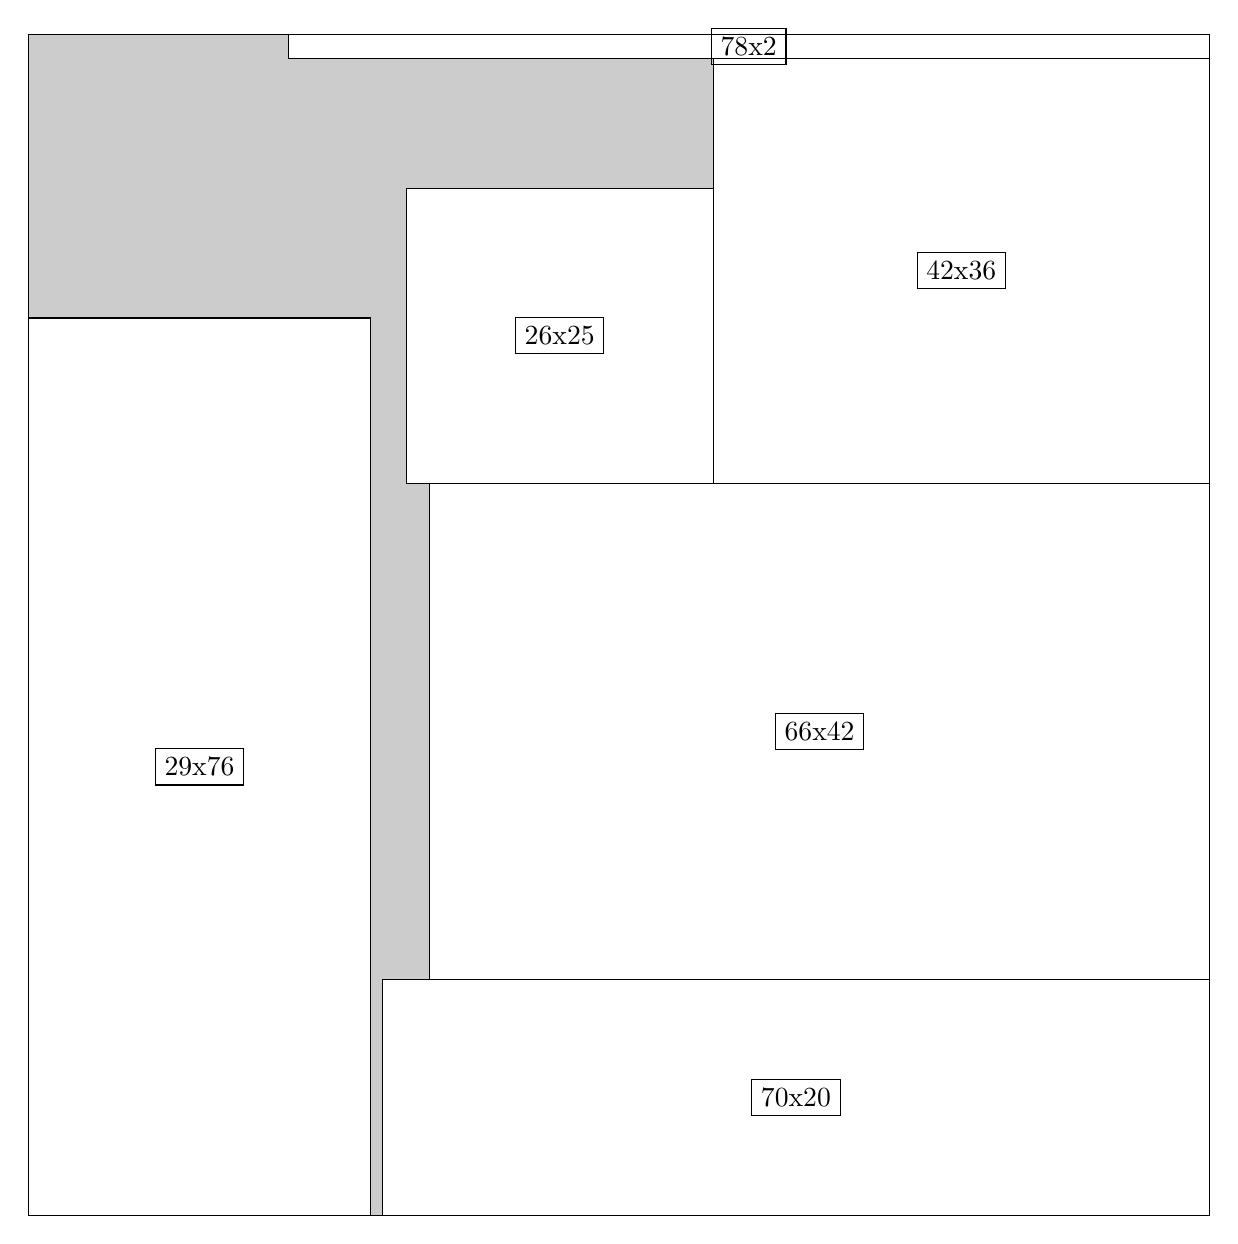
\begin{tikzpicture}[shorten >=1pt,scale=1.0,every node/.style={scale=1.0},->]
\tikzstyle{vertex}=[circle,fill=black!25,minimum size=14pt,inner sep=0pt]
\filldraw[fill=gray!40!white, draw=black] (0,0) rectangle (15.0,15.0);
\foreach \name/\x/\y/\w/\h in {70x20/4.5/0.0/10.5/3.0,66x42/5.1/3.0/9.9/6.3,42x36/8.7/9.299999999999999/6.3/5.3999999999999995,26x25/4.8/9.299999999999999/3.9/3.75,29x76/0.0/0.0/4.35/11.4,78x2/3.3/14.7/11.7/0.3}
\filldraw[fill=white!40!white, draw=black] (\x,\y) rectangle node[draw] (\name) {\name} ++(\w,\h);
\end{tikzpicture}


w =70 , h =20 , x =30 , y =0 , v =1400
\par
w =66 , h =42 , x =34 , y =20 , v =2772
\par
w =42 , h =36 , x =58 , y =62 , v =1512
\par
w =26 , h =25 , x =32 , y =62 , v =650
\par
w =29 , h =76 , x =0 , y =0 , v =2204
\par
w =78 , h =2 , x =22 , y =98 , v =156
\par
\newpage


\end{document}